\documentclass{VUMIFPSbakalaurinis}
\usepackage{algorithmicx}
\usepackage{algorithm}
\usepackage{algpseudocode}
\usepackage{amsfonts}
\usepackage{amsmath}
\usepackage{bm}
\usepackage{caption}
\usepackage{color}
\usepackage{float}
\usepackage{graphicx}
\usepackage{listings}
\usepackage{subfig}
\usepackage{wrapfig}

% Titulinio aprašas
\university{Vilniaus universitetas}
\faculty{Matematikos ir informatikos fakultetas}
\institute{Informatikos institutas}  % Užkomentavus šią eilutę – institutas neįtraukiamas į titulinį
\department{Programų sistemų bakalauro studijų programa}
\papertype{Bakalauro baigiamasis darbas}
\title{Krepšinio taisyklių pažeidimo automatinis nustatymas}
\titleineng{Recognizing violations of basketball rules using computer vision}
\author{Lukas Cedronas}
% \secondauthor{Vardonis Pavardonis}   % Pridėti antrą autorių
\supervisor{partn. prof., dr. Vytautas Ašeris}
\reviewer{lekt. Donatas Kimutis}
\date{Vilnius – \the\year}

% Nustatymai
% \setmainfont{Palemonas}   % Pakeisti teksto šriftą į Palemonas (turi būti įdiegtas sistemoje)
\bibliography{bibliografija}

\begin{document}
\maketitle

%% Padėkų skyrius
% \sectionnonumnocontent{}
% \vspace{7cm}
% \begin{center}
%     Padėkos asmenims ir/ar organizacijoms
% \end{center}

\sectionnonumnocontent{Santrauka}
Glaustai aprašomas darbo turinys: pristatoma nagrinėta problema ir padarytos
išvados. Santraukos apimtis ne didesnė nei 0,5 puslapio. Santraukų gale
nurodomi darbo raktiniai žodžiai. 
% Nurodomi iki 5 svarbiausių temos raktinių žodžių (terminų).
% Vienas terminas gali susidėti iš kelių žodžių.
\raktiniaizodziai{raktinis žodis 1, raktinis žodis 2, raktinis žodis 3, raktinis žodis 4, raktinis žodis 5}   

\sectionnonumnocontent{Summary}
Santrauka anglų kalba. Santraukos apimtis ne didesnė nei 0,5 puslapio.
\keywords{keyword 1, keyword 2, keyword 3, keyword 4, keyword 5}

\tableofcontents

\sectionnonum{Įvadas}
Įvade nurodomas darbo tikslas ir uždaviniai, kuriais bus įgyvendinamas tikslas,
aprašomas temos aktualumas, apibrėžiamas tiriamasis objektas akcentuojant
neapibrėžtumą, kuris bus išspręstas darbe, aptariamos teorinės darbo prielaidos
bei metodika, apibūdinami su tema susiję literatūros ar kitokie šaltiniai,
temos analizės tvarka, darbo atlikimo aplinkybės, pateikiama žinių apie
naudojamus instrumentus (programas ir kt., jei darbe yra eksperimentinė dalis).
Darbo įvadas neturi būti dėstymo santrauka. Įvado apimtis 2 –– 4 puslapiai.

\section{Naudoti įrankiai}

Kompiuterinės regos ir taisyklių pažeidimo atpažinimo algoritmams įgyvendinti buvo pasirinkta Python programavimo kalba. Python – interpretuojama, lengvai skaitoma kalba, puikiai tinkama įvairioms problemoms spręsti \cite{Python}. Dėl kalbos paprastumo ji dažnai naudojama kompiuterinės regos ir giliojo mokymo srityse, kadangi kalba leidžia susifokusuoti į abstrakcijas. Kadangi kalba yra plačiai naudojama, nesunku rasti daug pavyzdžių bei šaltinių. 

Objektų atpažinimui buvo pasirinkta OpenCV biblioteka. Tai – nemokama biblioteka, plačiai naudojama spręsti kompiuterinės regos uždavinius, kurios fokusas – įgalinti kurti aplikacijas leidžiančias efektyviai spręsti kompiuterinės regos problemas realiu laiku \cite{BradskiOpenCV}.

Vaizdo medžiaga rinkta filmuojant Xiaomi Redmi 8 Pro kamera.  

\section{Vaizdo medžiagos paruošimas}

Šio darbo metu sukurtai programinei įrangai paruošta vaizdo medžiaga, kurioje žaidėjas atlieka įvairius judesius su krepšinio kamuoliu. Siekiant supaprastinti vaizdo atpažinimo algoritmą, medžiagai keliami reikalavimai yra: aiškiai matomas žaidėjas, telpantis į kadrą ir užimantis nemažą dalį vaizdo. Vaizdo atpažinimui pagal spalvą algoritmui žaidėjas taip pat privalo dėvėti skirtingų spalvų pirštines, batus bei mušinėti atskiros spalvos kamuolį. Žaidėjas turi būti kiek galima labiau skirtis nuo fono, kad algoritmas veiktų kuo efektyviau, kadangi įvairių formų ir spalvų objektai fone pasunkina tikslų atpažinimą. Vaizdo medžiagoje žaidėjas mušinėja kamuolį ir atlieka įvairius judesius, dalis kurių pažeidžia taisykles, pavyzdžiui – pamušinėjęs kamuolį jį pasiima į rankas ir padaro keletą žingsnių. Programinė įranga turi atpažinti, jog tai – taisyklės pažeidimas. Vaizdo kokybė yra itin svarbi siekiant tikslių rezultatų, todėl buvo filmuojama kuo didesne raiška – Xiaomi Redmi Note 8 Pro kameros maksimali raiška yra 4K, 30 kadrų per sekundę. 

\section{Vaizdo atpažinimo metodai}

Vaizdo atpažinimas kompiuteriu yra vis dar problema. Egzistuoja daug algoritmų, kurių pagalba galima atpažinti objektus. Sudetingesniems objektams dažnai yra naudojami giliuoju mokymu paremti metodai, šiame darbe išnagrinėti keli iš jų. 
Atpažinti objektą reiškia priskirti jam kažkokį kontekstą. Tačiau kartais užtenka tiesiog 
//@todo Krepšinyje atpažinimas kažką pavaryti apie state of the art


\subsection{Spalvinis atpažinimas}
Vienas iš elementariausių būdų išskirti objektus ir priskirti jiems kontekstą yra tada, kai žinome jų spalvą iš anksto //@todo rasti kuo paremti. Tuomet pagal spalvų reikšmes nesunkiai galime išskirti regionus, juos reprezentuojant vienetukų ir nuliukų matricomis, ir atlikti įvairias logines operacijas. 

Tokio būdo trūkumas yra tai, jog norint panaudoti šį metodą atpažinti rankai ar kamuoliui, reikia iš anksto žinoti, kokios spalvos bus tie objektai. Negana to, labai sudėtinga išskirti atskiras kūno dalis naudojantis informacija apie odos spalvą, kadangi ne tik žaidėjo rankos, kojos bei veidas tikėtina bus tos pačios spalvos, bet galimai sutaps ir su kitų žaidėjų. 

Naudojantis spalvomis limitacijos yra labai aiškios... Siekiant ištirti spalvinių metodų efektyvumą ir pritaikomumą, būtina naudoti tam tikros spalvos pirštines, batus bei kamuolį, tačiau realiame pasaulyje žaidėjus priversti nešioti skirtingų spalvų batus, pirštines būtų itin nepraktiška. //@todo iškelti į išvadas ir pagrįsti Šie būdai tinkami tam tikrais išimtiniais atvejais. Šiame darbe taip pat bus nagrinėjami dar keli būdai, nepriklausantys nuo spalvų. 
\subsubsection{Segmentavimas}
Segmentavimą kompiuterinėje regoje galima suprasti kaip radimą grupės panašių pikselių. Kai paveikslėliai segmentuojami pagal spalvą, panašumą galima išmatuoti pagal reikšmių skirtumą RGB arba HSV modeliuose. Tai – gan paprastas būdas išskirti dominantį regioną, kadangi užtenka apsibrėžti tam tikrą intervalą spalvų, paveikslėlyje, reprezentuotame trimatine matrica, ir atfiltruoti matricos reikšmes nepatenkančias į duotąjį intervalą. 
RGB modelis, spalvą koduojantis trimis reikšmėmis, nusakančiomis raudonumą, žalsvumą ir mėlynumą. Turi trūkumą - keičiantis apšvietimui nenuspėjamai gali pasikeisti spalvos RGB reikšmė, kas filtravimą padaro itin sudėtingą. Problemą išssprendžia HSV modelis, kurio modelis spalvą reprezentuoja atspalviu, ryškumu ir šviesumu. HSV modelis puikiai tinka spalvų atpažinimui, kadangi H (atspalvio) reikšmė mažai kinta paveikslėliuose atsiradus šešėliams \cite{1039893} ar miglotumui \cite{7457892}. Atspalvis dažniausiai išlieka tas pats nepriklausomai nuo pašalinių efektų, todėl lengva nusistatyti reikšmių intervalą. Konvertavimas iš RGB ir HSV yra pakankamai trivialus, implementuotas cvtColor metodu. 

Turint intervalą užtenka atfiltruoti visus pikselius, kurių reikšmė nepatenka į duotą intervalą. Tiems, kurie patenka OpenCV priskiria 1, o kurie ne - 0. Rezultate gauname išskirtą regioną kur žinome, kad tai - tam tikra dalis, kadangi tik ji turėjo tą spalvą. //@todo style
\begin{figure}[H]
	\centering
	\subfloat[\centering Vaizdas prieš segmentavimo pagal pirštinės spalvą]{{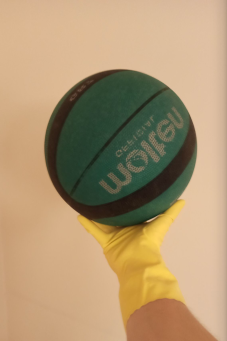
\includegraphics[width=5cm]{img/hand_before_segmentation} }}
	\qquad
	\subfloat[\centering Vaizdas po segmentavimo pagal pirštinės spalvą]{{
\includegraphics[width=5cm]{img/hand_after_segmentation} }}
	\caption{Fono Aaaa.}
	\label{fig:example}
\end{figure}

Šiame darbe naudojamų spalvų rėžiai //@todo add spalvos .  //@todo pagalvoti ar reikia <Pastebėta, jog lauke esančių paveikslėlių saturacija žymiai didesnė, nei kambaryje>

\subsubsection{Morfologinės transformacijos}
Atlikus segmentavimą pagal spalvą, rezultate dažnai lieka triukšmo ar bereikalingų artifaktų, kurie gali affectinti tolimesnį apdorojimą. @todo fix

Tokiais atvejais apsivalyti nuo triukšmo gan dažnai naudojamos slenkstinės (\textit{angl.} threshold) operacijos \cite[112]{SzeliskiCompVision}. Apsibrėžus tam tikrą filtrą, su juo galima atlikti operacijas ant matricų. Šiame darbe naudotos operacijos yra erozija ir plėstis. Erozija naudojama tada, norima sumažinti turimų atskirų regionų paveikslėlyje plotus, nuardant kraštus. Jei objektai yra pakankamai maži, o erozijos operacija - stipri (?), tuomet taip pašalinamas triukšmas. Formaliai erozija buvo aprašyta 1980 metais K. Y. Yoo \cite{4767941} kaip morfologinė operacija, sukombinuojanti dvi aibes naudojant vektorių atimtį aibių elementams. Matematiškai tai galima aprašyti tokia formule: 

\begin{equation}\label{eq:erozija}
	A \ominus B = \bigcap_ {b \in B } (A)_{-b} .
\end{equation}

\ref{eq:erozija} lygtyje A žymi dominantį paveikslėlį, išreikštą matrica, o B - filtrą arba kitaip - struktūrinį elementą, su kuriuo A matricoje pakartotinai atliekamos sankirtos.  

Erozijai priešinga operacija yra plėstis \ref{4767941}. Ši operacija leidžia padidinti išskirtų regionų plotą. Plėstis naudinga tuomet, kai po erozijos operacijos objektai praranda per daug ploto. Plėstį galima užrašyti šitaip:

\begin{equation}\label{eq:plestis}
	A \oplus B = \bigcup_ {b \in B } (A)_{b} .
\end{equation}

Atliekant bandymus pastebėta, jog siekiant geriausių rezultatų šalinant triukšmą, plėstį reikėtų vykdyti po erozijos, priešingu atveju triukšmas gali nebūti panaikintas. 

OpenCV įgyvendina funkcijas erode ir dilate, kurios priema paveikslėlio matricą ir struktūrinį elementą. Taip pat egzistuoja funkcija morphologyEx, kuri, priklausomai nuo paduodamų parametrų keičia savo veikimą: su MORPH\_OPEN atliekama plėstis po erozijos, su MORPH\_CLOSE - atvirkščiai. 

\subsubsection{Kamuolio kontūrų radimas}

//@todo pagalvoti ar prie spalvu turi eit
Siekiant iš paveikslikų išgauti daugiau kontekstualios informacijos, pavyzdžiui, ar kamuolys yra rankose, išsiskirti tarpusavy nesusikertančius regionus neužtenka. Tam, kad gauti šią informacijos dalį, reikia rasti, kada rankos ir kamuolio regionai susikerta, t.y. jų matricų sankirta yra netuščia. Tam reikia žinoti, kokią erdvę apima kamuolys - šios informacijos trūksta po segmentavimo pagal spalvą, jei kamuolys yra uždengtas, pavyzdžiui, rankos. 

Vienas iš būdų šią problemą išspręsti - pabandyti atspėti, kokią sritį užima kamuolys randant jo kontūrus. Skritulių kontūrams rasti 1991 metais E. Welzl pasiūlė algoritmą, rekursiškai apskaičiuojantį tam tikrai taškų aibei mažiausią ją apimantį apskritimą \cite{Welzl91smallestenclosing}. Šis algoritmas - tiesinio kompleksiškumo, jį įgyvendina OpenCV funkcija minEnclosingCircle().       

\begin{figure}[H]
	\centering
	\subfloat[\centering Kamuolio kontūrai prieš mažiausio aibę apimančio apskritimo radimo algoritmą]{{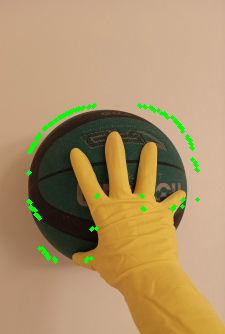
\includegraphics[width=5cm]{img/ball_contours_before} }}
	\qquad
	\subfloat[\centering Kamuolio kontūrai po mažiausio aibę apimančio apskritimo radimo algoritmo]{{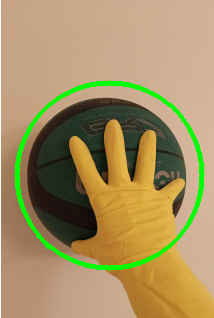
\includegraphics[width=5cm]{img/ball_contours_after} }}
	\caption{Fono Aaaa.}
	\label{fig:example}
\end{figure}

\subsection{Atpažinimas remiantis skirtumais}
\subsubsection{Fono pašalinimas}
Fono pašalinimas yra vienas iš esminių metodų kompiuterinėje regoje, naudojamas išskirti dominančius vaizdus ir pašalinti nereikalingus statiškus objektus iš fono. Pavyzdžiui, jei yra filmuojama lauke, fone besimatantys medžiai gali trukdyti tolimesniam atpažinimui, tad žinant, jog mus domina tik žaidėjas, pašalinius objektus galima pabandyti pašalinti. Vienas iš būdų yra iš anksto turėti fono paveiksliuką ir apdorojant kitus kadrus jį išimti, bet tai dažnai nepasiteisina dėl to, kad fonas gali kisti – gali atsirasti šešėlių, pasikeisti apšvietimas, gali būti įvairaus pašalinio judėjimo, pavyzdžiui – linguojantys medžiai, vaikštantys sirgaliai ir pan. 2002 m.  P. KaewTraKulPong pasiūlė algoritmą, išsprendžiantį šią problemą \cite{KaewTraKulPong2002}. Algoritmas kiekvieną pikselį sumodeliuoja į Gauso skirstinį pagal tai, kiek pikselio spalva keičiasi bėgant laikui. Kuo mažiau pikseliai keičiasi, tuo didesnė tikimybė, kad jie priklauso fonui. Naudojantis šiuo atradimu galima sėkmingai atsikratyti fono, taip išskiriant mus dominantį vaizdą. Šis metodas ypač tinkamas atpažinti judėjimui – vietoje stovintis žaidėjas bus priskirtas fonui, tačiau jam judant, lengvai galima išskirti jo siluetą.  

\begin{figure}[H]
    \centering
    \subfloat[\centering Vaizdas prieš fono pašalinimą.]{{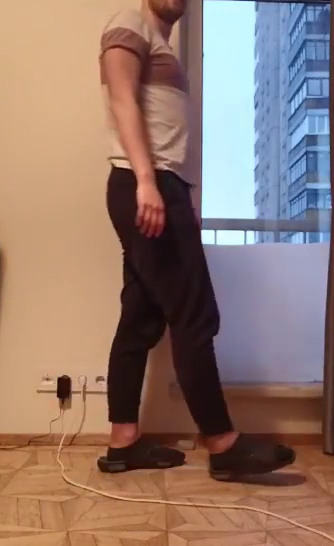
\includegraphics[width=5cm]{img/background-substraction-before} }}
    \qquad
    \subfloat[\centering Vaizdas po fono pašalinimo.]{{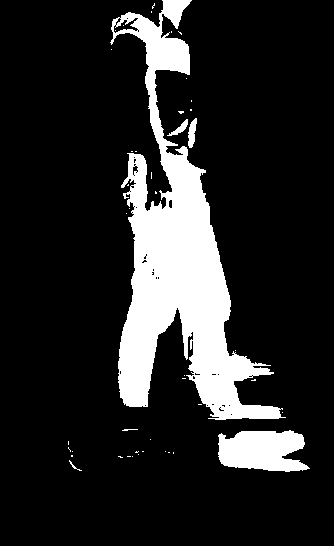
\includegraphics[width=5cm]{img/background-substraction} }}
    \caption{Fono pašalinimas naudojantis Gauso skirstiniu paremtu fono segmentavimo algoritmu.}
    \label{fig:example}
\end{figure}


Paveikslėlyje matome, jog algoritmas atpažino žmogaus siluetą. Šiame pavyzdyje ranka priskirta fonui dėl to, jog spalva sutampa su sienos spalva, tačiau kitos kūno dalys išskiriamos iš fono.

\subsubsection{Judesio atpažinimas}

Žaidėjui vaikštant, kai kurios kūno dalys juda greičiau, nei kitos. Kūnas išlieka santykinai statiškas palyginus su kojomis. Žingsniavimo mechanika yra tokia, kad atliekant žingsnį, viena koja lieka vienoje vietoje, kol kita yra perstatoma iš vienos pozicijos į kitą. Tam, kad pagauti tą kojos judesį, galima paprasčiausiai iš antro kadro atimti pirmą. Padalijus kadrą į dvi dalis – viršutinę ir apatinę – ir darant prielaidą, jog apatinėje dalyje matysis tik kojų judesiai, galima teigti, kad jei atėmus antrą kadrą iš pirmo yra skirtumas, buvo atliktas žingsnis. Koją pastačius ant žemės, tam tikrą laiką skirtumai sumažėja iki nustatytos ribos – pasinaudojus visa šia informacija galima apskaičiuoti, kiek žingsnių buvo atlikta. 

\begin{figure}[H]
    \centering
    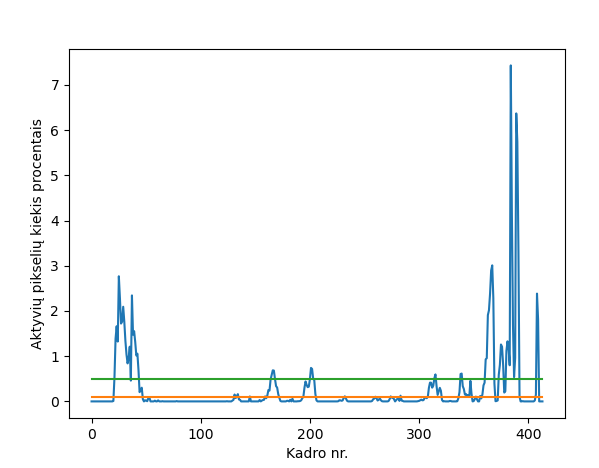
\includegraphics[scale=0.8]{img/steps}
    \caption{Aktyvių pikselių kiekis kiekviename kadre, indikuojantis žmogaus judėjimą. }
    \label{img:mlp}
\end{figure}

2 pav. pateiktoje lentelėje matyti, kiek buvo aktyvių pikselių kiekvieną kadrą panaudojus fono pašalinimą bei kadrų skirtumo algoritmus. Ši informacija rodo judėjimo kiekį tam tikrame kadro regione. Žalia linija žymi minimalų judėjimo kiekį, kuris gali atsirasti dėl triukšmo ir pašalinio judėjimo. Viršijus šią liniją galima teigti, jog žaidėjas juda. Oranžinė linija žymi ribą, kada galima sakyti, jog jokio judesio nėra, t.y. žaidėjas pastatė koją ir ruošiasi atlikti kitą žingsnį. 

\subsection{Žmogaus kūno dalių atpažinimas neuroniniais tinklais}

Šiuolaikinėje kompiuterinės regos srityje daug naudos galima gauti pasinaudojus neuroninių tinklų pagalba. Neuroniniai tinklai naudojami sprendžiant įvairias problemas, šiam darbui aktualiausia yra objektų atpažinimo problema. Turint tam tikrą kadrą, taisyklių pažeidimo algoritmui būtina, kad būtų atskirtos rankos, kojos ir kamuolys. Žmogaus kūno dalių klasifikavimas yra sudėtinga problema, kadangi dauguma algoritmų yra priklausomi nuo surinktų duomenų. Kompleksija tampa akivaizdi sprendžiant sporto problemas, kadangi labai dažnai žaidėjai daro įvairiausius judesius, apsirengę įvairiausiais rūbais ir pan., kas apsunkina žaidėjo kūno dalių atpažinimą \cite{Andriluka_2014_CVPR}. Tam reikalinga turtinga ir didelė duomenų aibė, dėl ko neuroninio tinklo apmokymo laikas išauga. 

Bene visi šiuolaikiniai metodai remiasi tuo pačiu principu: apmokinamas neuroninių tinklų modelis, jiems paruošiant teigiamus ir neigiamus pavyzdžius (pvz., siekiant sukurti kojų atpažinimo algoritmą, paveiksliukai, kuriuose yra koja pažymimi kaip teigiami, tie, kuriuose kojos nėra tampa neigiamais). Mokinimo procesas gali trukti daug laiko – kartais net savaites, todėl daug paprasčiau yra surasti jau sukurtą modelį ir jį pasinaudoti. Vienas iš modelių buvo pasiūlytas 2018 m., pavadinimu OpenPose \cite{cao2019openpose}. Modelio architektūra paremta konvoliuciniais neuroniniais tinklais. Modelis suskirstytas į dvi šakas. Viena jų priskiria tikimybes, kad tam tikras regionas yra tam tikra kūno dalis, kita – asociacijas tarp skirtingų kūno dalių. Atpažinimas vyksta keliais etapais, siekiant gauti kuo tikslesnius rezultatus. 

Šiame darbe kuriamas vaizdo atpažinimo algoritmas kiekvieną kadrą pateikia OpenPose modeliui, o rezultate gaunamos skirtingomis spalvomis sužymėtos kūno dalys. Taisyklių pažeidimo atpažinimo algoritmui aktualios yra rankų ir pėdų sritis. 

\begin{figure}[H]
    \centering
    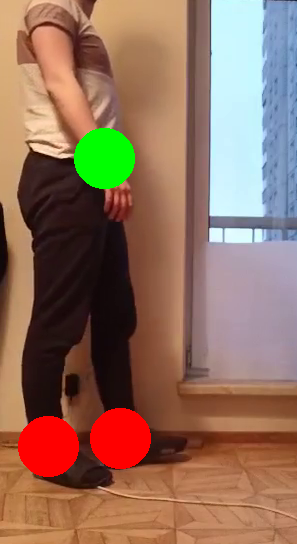
\includegraphics[scale=0.8]{img/body-parts}
    \caption{OpenPose algoritmo pagalba atpažintos kūno dalys.}
    \label{img:mlp}
\end{figure}

Vienas iš algoritmo trūkūmų yra tai, kad be optimizavimo su kiekvienu kadru gauti rezultatą užtrunka iki 0.5 sekundės. Galimas optimizavimo būdas yra sumažinti kadro dydį prieš pateikiant jį į neuroninį tinklą, tačiau tokiu atveju rezultatų tikslumas yra atvirkščiai proporcingas kadro dimensijom. 

\subsection{Kamuolio atpažinimas Hough Detection algoritmu}
@todo fix
Atpažinti kamuolį intitutyviai labai paprasta. Intuitive sako, jog reikia ieškoti apvalių kontūrų. Vienas iš nagrinėtų būdų – Hough Detection. Šį algoritmą natively supportina OpenCV. 

Hough Detection – trumpai aprašyti theory here

OpenCV turi metodą, įgyvendinantį algoritmą. 
Patikrinus algoritmą su vaizdo įrašu tapo akivaizdu, jog šis algoritmas tinka tik statiškam kamuoliui, o ne judančiam, kadangi jis visiškai praranda formą. 

\subsection{Body Part Segmentation}
@todo fix
Atpažinti kamuolį intitutyviai labai paprasta. Intuitive sako, jog reikia ieškoti apvalių kontūrų. Vienas iš nagrinėtų būdų – Hough Detection. Šį algoritmą natively supportina OpenCV. 

Hough Detection – trumpai aprašyti theory here

OpenCV turi metodą, įgyvendinantį algoritmą. 
Patikrinus algoritmą su vaizdo įrašu tapo akivaizdu, jog šis algoritmas tinka tik statiškam kamuoliui, o ne judančiam, kadangi jis visiškai praranda formą. 

\begin{figure}[H]
	\centering
	\subfloat[\centering Atrastas kamuolys]{{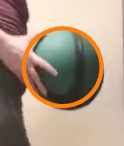
\includegraphics[width=5cm]{img/ball_circled} }}
	\qquad
	\subfloat[\centering Kamuolys deformuotas dėl judėjimo]{{
\includegraphics[width=5cm]{img/ball_notfound} }}
	\caption{Fono Aaaa.}
	\label{fig:example}
\end{figure}

\sectionnonum{Rezultatai ir išvados}
Rezultatų ir išvadų dalyje išdėstomi pagrindiniai darbo rezultatai (kažkas
išanalizuota, kažkas sukurta, kažkas įdiegta), toliau pateikiamos išvados
(daromi nagrinėtų problemų sprendimo metodų palyginimai, siūlomos
rekomendacijos, akcentuojamos naujovės). Rezultatai ir išvados pateikiami
sunumeruotų (gali būti hierarchiniai) sąrašų pavidalu. Darbo rezultatai turi
atitikti darbo tikslą.

\printbibliography[heading=bibintoc]  % Šaltinių sąraše nurodoma panaudota
% literatūra, kitokie šaltiniai. Abėcėlės tvarka išdėstomi darbe panaudotų
% (cituotų, perfrazuotų ar bent paminėtų) mokslo leidinių, kitokių publikacijų
% bibliografiniai aprašai. Šaltinių sąrašas spausdinamas iš naujo puslapio.
% Aprašai pateikiami netransliteruoti. Šaltinių sąraše negali būti tokių
% šaltinių, kurie nebuvo paminėti tekste. Šaltinių sąraše rekomenduojame
% necituoti savo kursinio darbo, nes tai nėra oficialus literatūros šaltinis.
% Jei tokių nuorodų reikia, pateikti jas tekste.

% \sectionnonum{Sąvokų apibrėžimai}
\sectionnonum{Santrumpos}
Sąvokų apibrėžimai ir santrumpų sąrašas sudaromas tada, kai darbo tekste
vartojami specialūs paaiškinimo reikalaujantys terminai ir rečiau sutinkamos
santrumpos.

\appendix  % Priedai
% Prieduose gali būti pateikiama pagalbinė, ypač darbo autoriaus savarankiškai
% parengta, medžiaga. Savarankiški priedai gali būti pateikiami ir
% kompaktiniame diske. Priedai taip pat numeruojami ir vadinami. Darbo tekstas
% su priedais susiejamas nuorodomis.

\section{Neuroninio tinklo struktūra}
\begin{figure}[H]
    \centering
    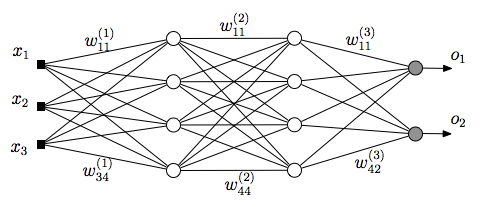
\includegraphics[scale=0.5]{img/MLP}
    \caption{Paveikslėlio pavyzdys}
    \label{img:mlp}
\end{figure}


\section{Eksperimentinio palyginimo rezultatai}
% tablesgenerator.com – converts calculators (e.g. excel) tables to LaTeX
\begin{table}[H]\footnotesize
  \centering
  \caption{Lentelės pavyzdys}
  {\begin{tabular}{|l|c|c|} \hline
    Algoritmas & $\bar{x}$ & $\sigma^{2}$ \\
    \hline
    Algoritmas A  & 1.6335    & 0.5584       \\
    Algoritmas B  & 1.7395    & 0.5647       \\
    \hline
  \end{tabular}}
  \label{tab:table example}
\end{table}

\end{document}
